\documentclass[]{article}
\usepackage[utf8]{inputenc} 
\usepackage[T1]{fontenc}
\usepackage{lmodern}
\usepackage[ngerman]{babel}
\usepackage{courier}
\usepackage{amsmath}
\usepackage{multicol}
\usepackage[top=2cm, bottom=2cm, left=2cm, right=2cm]{geometry}
\usepackage{authblk}
\usepackage[font=scriptsize, labelfont=bf]{caption}
\usepackage{listings}
\usepackage{hyperref}
\usepackage{color}
\usepackage{float}
\usepackage{amssymb}
\usepackage{graphicx, caption}
\usepackage{sidecap}
\usepackage{flafter}  
\usepackage[style=numeric]{biblatex}
\usepackage[babel,german=guillemets]{csquotes}
\bibliography{literatur}
\usepackage{bbm}
\definecolor{dkgreen}{rgb}{0,0.6,0}
\definecolor{gray}{rgb}{0.5,0.5,0.5}
\definecolor{mauve}{rgb}{0.58,0,0.82}

\lstset{frame=tb,
  language=C,
  aboveskip=3mm,
  belowskip=3mm,
  showstringspaces=false,
  columns=flexible,
  basicstyle={\small\ttfamily},
  numbers=none,
  numberstyle=\tiny\color{gray},
  keywordstyle=\color{blue},
  commentstyle=\color{dkgreen},
  stringstyle=\color{mauve},
  breaklines=true,
  breakatwhitespace=true,
  tabsize=3
  }
\captionsetup{width=1\linewidth}

% for skript letters like H...
\usepackage{mathrsfs}
\usepackage{fancyhdr}
\fancyhf{}
\fancyfoot[LE,RO]{\thepage}
\usepackage{hyperref}
\pagestyle{fancy}
\geometry{verbose,a4paper,tmargin=25mm,bmargin=25mm,lmargin=15mm,rmargin=20mm}



\title{Protocol}

\author{Nicolas Heimann}
\affil{nicolas.heimann@studium.uni-hamburg.de}
\author{Jesse Hinrichsen}
\affil{jesse.hinrichsen@studium.uni-hamburg.de}
\date{07.03. - 12.03.2016}
\affil{Universität Hamburg}
\begin{document}
\begin{titlepage}
\maketitle
\thispagestyle{empty}
\end{titlepage}
\pagebreak
\abstract{
An abstract...
}
\tableofcontents
\pagebreak
\section {Introcution}

\section{Identifying events}
Quantities for events:
\newline
Ctrk(Sump): Energy of charged traces
\newline
Ctrk(N): Number of charged traces 
\newline
Ecal(SumE): Energy in electronic-kalorimeter
\newline
Hcal(SumE): Energy in hadronic-kalorimeter

\begin{tabular}{ |p{1cm}||p{2cm}|p{3cm}|p{3cm}|p{3cm}|p{3cm}|  }
 \hline
 \multicolumn{6}{|c|}{Quantities} \\
 \hline
 Run & Event & Ctrk(Sump) & Ctrk(N) & Ecal(SumE) & Hcal(SumE) \\
 \hline
 00 & ELECTRONS   & AF    &AFG&   004 & 00\\
 00 & MUONS & AF    &AFG&   004 & 00\\
 00 & TAUS & AF    &AFG&   004 & 00\\
 00 & HADRONS    & AF    &AFG&   004 & 00\\
 \hline
\end{tabular}

\section {Statistical analysis of $Z^0$ decay channels}

\subsection{Decay width and cross-section}
Using equation (2.12) we calculate following decay width of the Z-boson into fermions and (2.14) for cross-section at peak.

\begin{tabular}{ |p{3cm}||p{3cm}|  }
 \hline
 \multicolumn{2}{|c|}{Decay width for different channels} \\
 \hline
 Channel & Decay width \\
 \hline
  $\Gamma_l = \Gamma_e = \Gamma_{\mu} = \Gamma{\tau} $   & 85.9 MeV   \\
  $\Gamma_{\nu} $   & 165.9 MeV   \\
  $\Gamma_u = \Gamma_c $   & 301.5 MeV   \\
  $\Gamma_d = \Gamma_s = \Gamma_b $   & 381.4 MeV   \\
  \hline
  $\Gamma_Z $   & 2502.7 MeV   \\
  $\Gamma_{hadr} $   & 1747.3 MeV   \\
  $\Gamma_{lept}\footnote{Without neutrinos} $   & 257.8  MeV   \\
  $\Gamma_{neutr} $   & 497.6  MeV   \\
 \hline
 \hline
 \multicolumn{2}{|c|}{Partial cross-section at peak} \\
 \hline
  $\sigma_{lept} $   & 5.35 $KeV^{-2}$   \\
  $\sigma_{neutr} $   & 10.32 $KeV^{-2}$   \\
  $\sigma_{u, c} $   & 18.76 $KeV^{-2}$   \\
  $\sigma_{d,s,c} $   & 23.73 $KeV^{-2}$   \\
 \hline
\end{tabular}

\subsection{Estimating change of $Z^0$ decay width for additional channels}

\begin{tabular}{ |p{3cm}||p{3cm}|p{3cm}|  }
 \hline
 \multicolumn{3}{|c|}{Decay width of $Z^0$ for additional channels} \\
 \hline
 Added channel & $Z^0$ width & relative increase \\
 \hline
   Lepton & 2.589 GeV & 3.5 \%  \\
   Neutrino & 2.669  GeV & 6.6 \%  \\
   u-Quark & 2.804  GeV & 12 \%  \\
   d-Quark & 2.884 GeV & 15.2 \%  \\
  \hline
\end{tabular}

\subsection{Differential cross-section}
\begin{figure}[H]
	\centering
	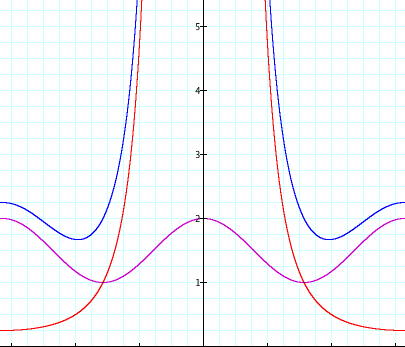
\includegraphics[scale=0.4]{differential-cross-section}
	\caption{Differential cross-section on $\Theta$ qualitatively. Red: t-channel, violet: s-channel, blue: s-channel + t-channel}
	\label{fig:diff-cross-section}
\end{figure}
For s-channel: $\frac{d\sigma}{d\Omega} \propto 1 + \cos^2{\Theta}$ (for big $Theta$)
\newline
For t-channel: $\frac{d\sigma}{d\Omega} \propto (1 - \cos{\Theta})^{-2}$ (for small $Theta$)

\subsection{Forward-Backward Asymmetry}
Based on equation (2.18)
\begin{tabular}{ |p{3cm}||p{2cm}|p{2cm}|p{2cm}|  }
 \hline
 \multicolumn{4}{|c|}{Forward-Bckward asymmetry} \\
 \hline
 $\sqrt{s}$ / $\sin^2(\theta_W)$ & 0.21 & 0.23 & 0.25 \\
 \hline
   89.225 GeV & 0.547 & 0.321 & 0.285  \\
   91.225 GeV & 0.530 & 0.407 & 0.284  \\
   93.225 GeV & 0.515 & 0.480 & 0.284  \\
  \hline
\end{tabular}
\begin{figure}[H]
	\centering
	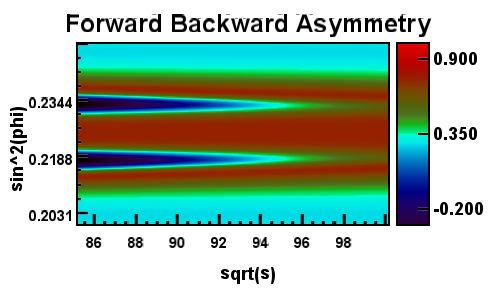
\includegraphics[scale=0.4]{forward_backward_symmetry}
	\caption{Forward-Bckward asymmetry}
	\label{fig:for-back-asy}
\end{figure}



\pagebreak
\nocite{*}
\printbibliography



\end{document}